\documentclass[a4paper,10pt,fleqn]{article}
\usepackage[dvipdfmx]{graphicx}
\title{{\Huge Capstone Project}}%%% \\Machine Learning Engineer Nanodegree}

\author{Ryosuke Honda}
\date{\today}
\begin{document}
\maketitle

\section{Definition}
\subsection{Project Overview}
Student provides a high-level overview of the project in layman’s terms. Background information such as the problem domain, the project origin, and related data sets or input data is given.


The improvement on the camera and the widespread of larger capacity hardwares lead us to store more digital pictures. However computers can't understand the meaning of the pictures, so it is essential for us humans to classify or search images. Image recognition(Figure.\ref{fig:one}) will help us to classify or search pictures without our intervention. These days, because of the development of the computational capacity, we can process large number of pictures with high level accuracy(nearly the human's recognition). In this project, I'll discuss the image recognition algorithm which will be useful in the classification of large number of images.


\begin{figure}[htbp]

\begin{center}
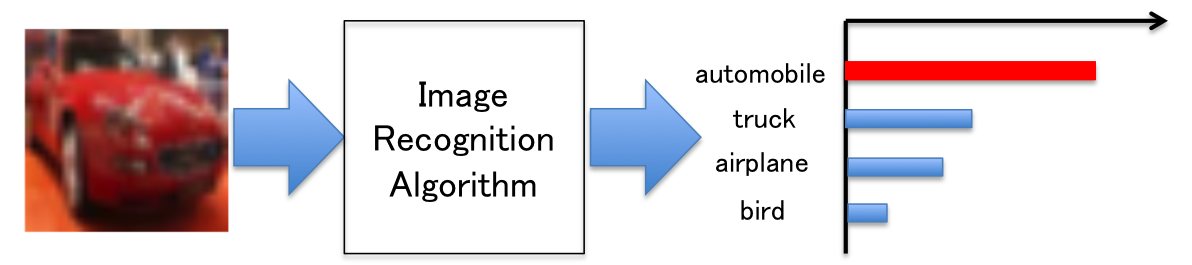
\includegraphics[width=10cm]{picture/Image_Recognition.png}
\end{center}
\caption{Image of the Algorithm}
\label{fig:one}

\end{figure}



\subsection{Problem Statement}
The problem which needs to be solved is clearly defined. A strategy for solving the problem, including discussion of the expected solution, has been made.







{\Large The CIFAR-10 dataset}\\
The CIFAR-10 dataset consists of 60,000 32x32x3(width=height=32 and RGB=3) color images in 10 classes, with 6,000 images. 50,000 images are the training images and 10,000 images are the test images.\\
The classes are completely mutually exclusive. There is no overlap within each image class.

In this task, I'll discuss the image recognition by Convolutional Neural Network(CNN).





\subsection{Metrics}
Metrics used to measure performance of a model or result are clearly defined. Metrics aper classre justified based on the characteristics of the problem.


The objective in this problem is multi class classification. Therefore,the metrics will be 'cross entropy'.
Cross entropy is 


\section{Analysis}
\subsection{Data Exploration}
If a dataset is present, features and calculated statistics relevant to the problem have been reported and discussed, along with a sampling of the data. In lieu of a dataset, a thorough description of the input space or input data has been made. Abnormalities or characteristics about the data or input that need to be addressed have been identified.


CIFAR-10 dataset consists of 50,000 images of training data and 10,000 images of test data.For each data, it contains 10 different kind of classes(discussed in the next chapter) and the distribution of each class is the same in both training and test data. That means 5,000 images for each class in the training data and 1,000 images for each class in the test data.(Figure.\ref{fig:three} and Figure.4). 


\subsection{Exploratory Visualization}
A visualization has been provided that summarizes or extracts a relevant characteristic or feature about the dataset or input data with thorough discussion. Visual cues are clearly defined.


There are 60,000 of images in total. Figure(50,000 images for training data and 10,000 images for test data).\ref{fig:two} shows the samples of the images. I plotted 10 images for each class.Figure.\ref{fig:three} and Figure.\ref{fig:four} shows the distribution of the data. For the training dataset, each class has 5,000 images and for the test dataset, each class has 1,000 images.
The label 0 to 9 corresponds to 'Airplane','Automobile','Bird','Cat','Deer','Dog','Frog','Horse','Ship, and 'Truck'.
\begin{figure}[htbp]

\begin{center}
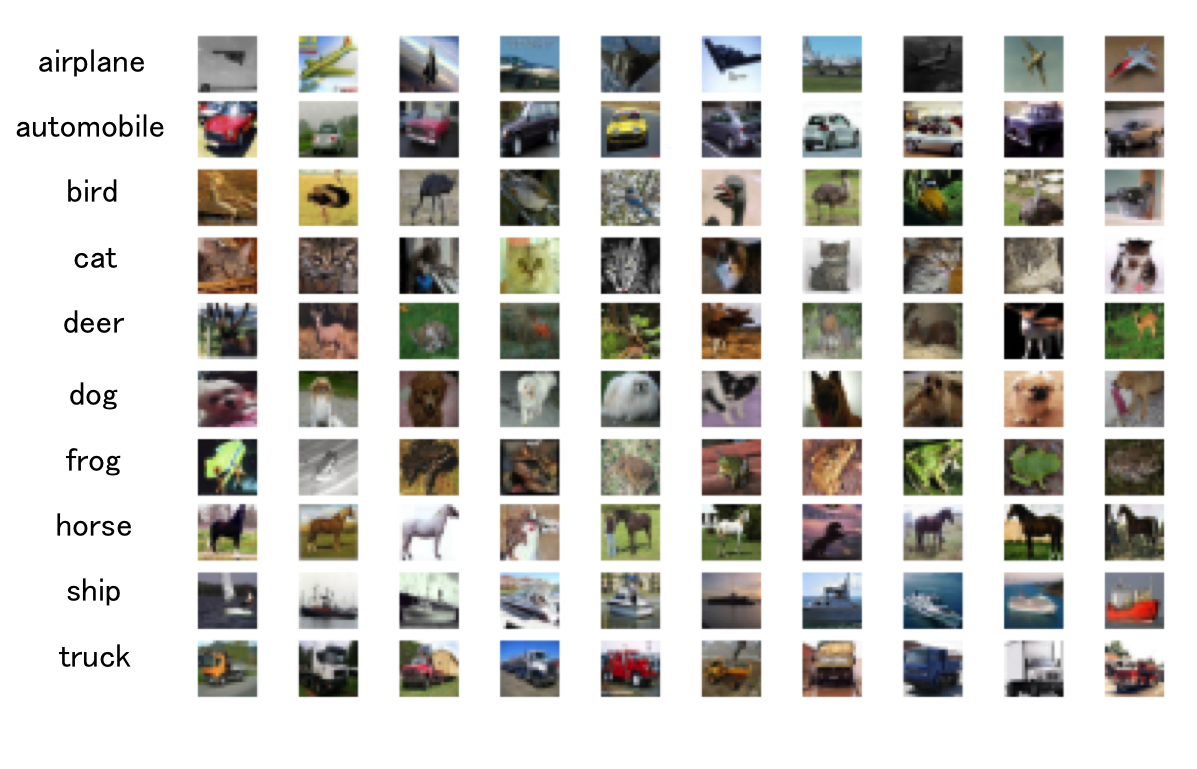
\includegraphics[width=10cm]{picture/random_sample.png}
\end{center}
\caption{Sample of the Images}
\label{fig:two}

\end{figure}

\begin{figure}[h]
\begin{minipage}{0.5\hsize}
	\begin{center}
	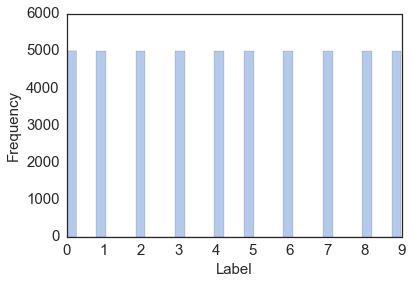
\includegraphics[width=5cm]{picture/Distribution_of_Training_Data.png}
	\end{center}
	\caption{Distribution of Training Data}
	\label{fig:three}
\end{minipage}
\begin{minipage}{0.5\hsize}
\begin{center}
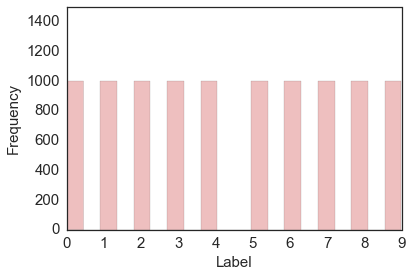
\includegraphics[width=5cm]{picture/Distribution_of_Test_Data.png}
\end{center}
 \caption{Distribution of Test Data}
  \label{fig:four}
 \end{minipage}
\end{figure}


\subsection{Algorithms and Techniques}
Algorithms and techniques used in the project are thoroughly discussed and properly justified based on the characteristics of the problem.

In this task, I'll use Convolutional Neural Network(CNN). CNN has been successful in  practical applications for image recognition.CNN consists of convolution layer, pooling layer and fully-connected layer and sometimes contains local contrast normalization(LCN). In this chapter, I'll discuss the convolution layer and pooling.
As the name 'convolution' suggests, the network employs a mathematical operation called convolution. 

Figure.5 is the example of the architecture of the CNN.
\begin{figure}[htbp]

	\begin{center}
	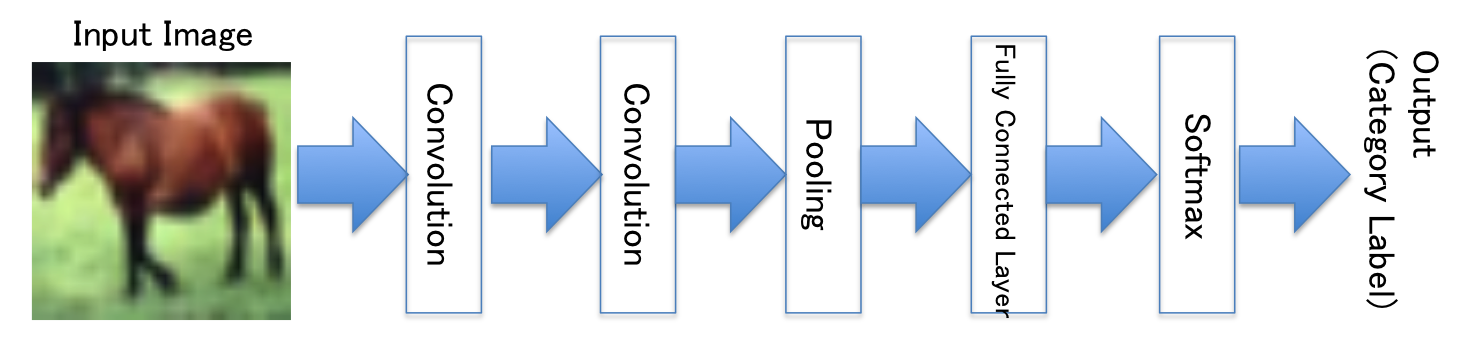
\includegraphics[width=10cm]{picture/Architecture_of_CNN.png}
	\caption{An example of CNN Architecture}
	\end{center}
	\label{fig:five}

\end{figure}



\subsection{Benchmark}
Student clearly defines a benchmark result or threshold for comparing performances of solutions obtained.


\section{Methodology}
\subsection{Data Preprocessing}
All preprocessing steps have been clearly documented. Abnormalities or characteristics about the data or input that needed to be addressed have been corrected. If no data preprocessing is necessary, it has been clearly justified.


\subsection{Implementation}
The process for which metrics, algorithms, and techniques were implemented with the given datasets or input data has been thoroughly documented. Complications that occurred during the coding process are discussed.

\subsection{Refinement}
The process of improving upon the algorithms and techniques used is clearly documented. Both the initial and final solutions are reported, along with intermediate solutions, if necessary.



\section{Result}
\subsection{Model Evaluation and Validation}
The final model’s qualities — such as parameters — are evaluated in detail. Some type of analysis is used to validate the robustness of the model’s solution.

\subsection{Justification}
The final results are compared to the benchmark result or threshold with some type of statistical analysis. Justification is made as to whether the final model and solution is significant enough to have adequately solved the problem.




\section{Conclusion}
\subsection{Free-Form Visualization}
A visualization has been provided that emphasizes an important quality about the project with thorough discussion. Visual cues are clearly defined.

\subsection{Reflection}
Student adequately summarizes the end-to-end problem solution and discusses one or two particular aspects of the project they found interesting or difficult.

\subsection{Improvement}
Discussion is made as to how one aspect of the implementation could be improved. Potential solutions resulting from these improvements are considered and compared/contrasted to the current solution.





\end{document}